% (c) 2026 Stephanie Märklin, OST Ostschweizer Fachhochschule
%
% !TEX root = ../../buch.tex
% !TEX encoding = UTF-8
%
% Rolle im Paper: Konkretisierung des Problems. Das allgemeine Problem auf
% einen konkreten,% behandelbaren Fall eingrenzen und die Wahl begründen
%
% Stichworte:
% 17.1 Grundbegriffe
% - welche Begriffe folgen und wozu (Werkzeugkasten für die Leitfrage)
% - Achsen benennen: Rollen/Längsachse, Nicken/Querachse, Gieren/Hochachse
% - Ruhelage konkret: getrimmter Geradeausflug; Störung: Böe
% - Definition stabil: selbständige Rückkehr, ohne Piloteneingriff
%   (stick fixed), auf allen drei Achsen
%
% 17.1.1 Stabilität
% - Kernpunkt: Stabilität ist eine Eigenschaft des Flugzeugs selbst --
%   sie entsteht durch die Konstruktion (Geometrie, Leitwerk) und
%   bestimmt Einsatz und Handhabung
% - Anknüpfen: Definition aus 17.1 ist qualitativ (stabil ja/nein)
% - Konkretisierung: ja/nein nicht genug für die Eigenschaft
%   wir müssen wissen OB und WIE schnell die Bewegung abklingt
% - Problem: Erfliegen/Beobachten liefert die Antwort erst, wenn das
%   Flugzeug existiert, das ist zu spät
% - Folgerung: wir müssen die Bewegung nach der Störung berechnen können
%   (Leitfrage konkretisiert)
% - Übergang: dazu braucht es eine mathematische Beschreibung der
%   Bewegung -> Aufzeigen anhand der Dutchroll (führt zu 17.1.2)

% Stichworte:
% 17.1.2 Die Dutch Roll
% - Phänomen beschreiben: Nase schwingt links-rechts, Flügel wippen
%   gegenphasig (Verweis auf Abbildung?)
% - Mechanismus verbal als Kreislauf: Gieren erzeugt Schieben,
%   Schieben erzeugt Rollen, Rollen erzeugt Gieren
% - dabei: Schieben ist NEU -- keine Drehbewegung, sondern seitliche
%   Bewegung; kurz einführen (ein Satz), formal als Schiebewinkel
%   erst in 17.2
% - Pointe: die Bewegungen sind gekoppelt -- keine Achse lässt sich
%   allein betrachten
% - Schluss (Übergang): ob die Schwingung abklingt und wie schnell,
%   lässt sich am Phänomen nicht ablesen -- dafür brauchen wir die
%   Grössen, die die Bewegung beschreiben (-> 17.2)

\section{Grundbegriffe der Flugstabilität
\label{aircraft:section:1-grundbegriffe}}
\kopfrechts{Grundbegriffe}
Um die Stabilität eines Flugzeugs beschreiben zu können, führen wir zunächst
die drei Flugzeugachsen und ihre Drehbewegungen ein.
Die Abbildung~\ref{aircraft:fig:achsen} zeigt die drei Achsen mit den
zugehörigen Drehbewegungen.
Das \emph{Nicken} (pitch) ist die Drehbewegung um die Querachse, das
\emph{Rollen} (roll) die Drehbewegung um die Längsachse und das \emph{Gieren}
(yaw) die Drehbewegung um die Hochachse.
\input{papers/aircraft/fig/fig-achsen}
Als Ruhelage betrachten wir den getrimmten Geradeausflug:
Die Flügel liegen horizontal, das Flugzeug nickt und giert nicht.
Eine Störung wie eine Böe bewegt das Flugzeug aus der Ruhelage.
Das Flugzeug heisst stabil, wenn es ohne Eingriff des Piloten in die
Ruhelage zurückkehrt.

\subsection{Stabilität als Flugzeugeigenschaft
\label{aircraft:subsection:eigenschaft}}
Die Stabilität ist eine Eigenschaft des Flugzeugs selbst.
Sie beeinflusst unter anderem dessen Handhabung und Agilität.
Bestimmt wird sie durch die Konstruktion und damit bereits im Entwurf.

Die Definition aus Abschnitt~\ref{aircraft:section:1-grundbegriffe}
beurteilt die Stabilität nur qualitativ.
Das Flugzeug kehrt in die Ruhelage zurück oder nicht.
Für die Konstruktion müssen wir wissen, ob das Flugzeug zurückkehrt und wie
schnell die Bewegung abklingt.
Die Ermittlung durch Messungen liefert diese Antwort erst, wenn das
Flugzeug gebaut ist, und damit zu spät für den Entwurf.
Wir müssen die Bewegung nach einer Störung bereits vorher berechnen können.
Welche Grössen diese Bewegung beschreiben, zeigt sich an einem Phänomen,
bei dem sich die Drehbewegungen gegenseitig beeinflussen: der Dutch Roll.

\subsection{Die Dutch Roll
\label{aircraft:subsection:dutchroll}}
Die \emph{Dutch Roll} ist ein charakteristisches Schwingungsmuster.
Die Abbildung~\ref{aircraft:fig:dutchroll} zeigt ihren Ablauf.
%! Author = stephaniemaerklin
%! Date = 30.08.2026

\begin{figure}
    \centering
    \includegraphics[width=0.7\textwidth]{papers/aircraft/images/dutchroll.png}
    \caption{Ablauf der Dutch Roll.
    Oben die Vorderansicht, das Flugzeug rollt abwechselnd nach rechts und
    nach links, die punktierte Linie ist die Flugbahn.
    Unten die Draufsicht, das Flugzeug fliegt von rechts nach links, die Nase
    pendelt um die Flugrichtung, das Flugzeug giert und schiebt.
    \label{aircraft:fig:dutchroll}}
\end{figure}
Eine Störung dreht die Nase nach links (1).
Der rechte Flügel senkt sich (2), und die Nase dreht zurück nach
rechts (3).
Darauf senkt sich der linke Flügel (4), und die Nase dreht erneut
nach links (5).
Das Flugzeug überschiesst die Ruhelage.
Es entsteht eine Schwingung.
In den Drehbewegungen ausgedrückt heisst das:
Gieren erzeugt Schieben, Schieben erzeugt Rollen, und Rollen erzeugt
erneut Gieren.
Dabei bezeichnet \emph{Schieben} (sideslip), dass die Bewegungsrichtung des
Flugzeugs von seiner Längsachse abweicht.

% QR-CODE 1 (Herausgeber): rechts neben diesem Absatz
% Ziel: https://www.youtube.com/watch?v=9Gt-IcCBiQ4
% Beschriftung: Vorschlag "Video: Erklärung Dutch Roll (en)"
%
% videoqrcode.tex
%
% (c) 2026 Prof Dr Andreas Müller
%
\vspace*{-12pt}
\smash{\hbox to12.26cm{\hfill\raisebox{-2.2cm}{%
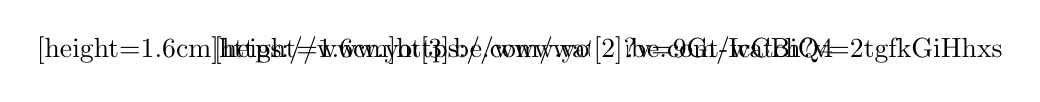
\begin{tikzpicture}
\node at (-1.1,0) {\qrcode[height=1.6cm]{https://www.youtube.com/watch?v=9Gt-IcCBiQ4}};
\fill[color=white] (-1.1,0) circle[radius=0.24];
\node at (-1.1,0) {[3]};
\node at (1.1,0) {\qrcode[height=1.6cm]{https://www.youtube.com/watch?v=2tgfkGiHhxs}};
\fill[color=white] (1.1,0) circle[radius=0.24];
\node at (1.1,0) {[2]};
\end{tikzpicture}
}}}%
\hangindent=-4.4cm
\hangafter=-6

\phantom{000}Das Video \cite{aircraft:video-erklaerung} zeigt diesen Ablauf in Bewegung.
Es erklärt zusätzlich, welche Eigenschaften des Flugzeugs die Schwingung
begünstigen; darauf kommen wir in Abschnitt 17.7 zurück.
%
%
% QR-CODE 2 (Herausgeber): rechts neben diesem Absatz
% Ziel: https://www.youtube.com/watch?v=2tgfkGiHhxs
% Beschriftung: Vorschlag "Video: Aufnahme Dutch Roll"
Wie intensiv eine Dutch Roll ausfallen kann, zeigt die Aufnahme
\cite{aircraft:video-aufnahme} eines dreistrahligen Verkehrsflugzeugs.

Die Dutch Roll ist eine von drei Bewegungsformen, mit denen ein
Flugzeug auf eine Störung der \emph{Seitenbewegung} (lateral motion) antwortet.
Die Seitenbewegung umfasst das Gieren, das Schieben und das Rollen.
Die \emph{Rollbewegung} (roll mode) ist eine Drehung um die Längsachse.
Der absinkende Flügel erzeugt dabei mehr Auftrieb als der steigende und bremst
die Drehung.
Bei gewöhnlichen Anstellwinkeln klingt die Rollbewegung deshalb rasch ab.
Die \emph{Spiralbewegung} (spiral mode) verläuft ohne Schwingung.
Das Flugzeug neigt sich langsam zur Seite, die Nase dreht in die Kurve, und der
Rollwinkel wächst weiter.
Ob die Spiralbewegung abklingt oder anwächst, hängt von der Konstruktion ab.
In beiden Fällen ist die Bewegung so langsam, dass der Pilot sie leicht
korrigieren kann.
Die Dutch Roll dagegen ist eine Schwingung, bei der offen bleibt, ob sie
abklingt und wie schnell.
Im Folgenden untersuchen wir deshalb die Dutch Roll.

Ob die Schwingung abklingt und wie schnell, lässt sich am Schwingungsmuster
nicht direkt ablesen.
Dafür brauchen wir Grössen, die die Bewegung beschreiben.
